\chapter{Hardware}
\section{Inverted pendulum}
\section{Controller}

\chapter{Software}


\chapter{Controllers}
\section{Linear quadratic regulator (LQR)}
\subsection{Theory}
The Linear Quadratic Regulator (LQR) has been presented by Rudolf E. Kalmanin in 1960 \cite{lqrLecture}. This optimal control algorithm is used for stabilizing linear dynamic systems by determining a control input that minimizes a quadratic cost function. LQR is an unified systematic control method for multiple-input multiple-output (MIMO) systems \cite{lqrLecture}. It is a very popular control algorithm because of its inherent robustness, where the gain and phase margin are guaranteed \cite{1102565}. 

Central to the LQR framework is the concept of linear system dynamics. LQR is tailored for linear time-invariant systems, typically characterized by matrices A, B, C, and D, encapsulating the system's behavior \cite{wikiLQR}.

At its core, LQR revolves around the minimization of a quadratic cost function over a specified time horizon. LQR reduces the amount of labor that needs to be put into the design of the controller, although the formulation of the cost function plays a crucial role in the controller performance.

The solution to the LQR problem involves online and offline calculations that can be separated to three distinct parts \cite{lqrLecture}:
\textbf{
\begin{enumerate}
	\item Solving the Riccati differential equation \footnote{Riccati differential equation is a type of first-order ordinary differential equation that has a quadratic term in one of its variables} 
	\item Computation of the feedback matrix K*\(t\)
	\item Evaluation of the feedback control law
\end{enumerate}
} 

Linear quadratic control problem can be formulated as Eq. \ref{eq1}
\begin{equation}\label{eq1}
\underset{x(t),u(t).t_e}{min}J(x(t),u(t),t_e)\: with \: J=\frac{1}{2}x(t_e)^TSx(t_e)+\frac{1}{2}\int_{0}^{t_e}x(t)^TQ(t)x(t)+u(t)^TR(t)u(t)dt
\end{equation}
where $x(t_e)$ is the end state vector, $Q(t)$ is the state weighting matrix, $R(t)$ is the input weighting matrix and $S$ is the end weighting matrix. Weighting matrices $Q,R$ and $S$ are design parameters and with the help of them, we can change the behavior of the controller. The optimal feedback control law is give by Eq. \ref{eq2} \cite{lqrLecture}

\begin{equation}\label{eq2}
u^*(t)=K^*(t)x(t)
\end{equation}

where $K^*$ is the feedback matrix. given by Eq. \ref{eq3} \cite{lqrLecture}
\begin{equation}\label{eq3}
K^*(t)=R(t)^{-1}B(t)^TP(t)
\end{equation}

\subsection{Simulation}
In the context of simulation using MATLAB for control system design, the provided code, obtained from the lab coordinator, incorporates the design of a Linear Quadratic Regulator (LQR) controller used for the control of nonlinear inverted pendulum. The primary objective is to evaluate the functionality of the code under different conditions. To assess the system's robustness and performance, disturbances have been introduced. Additionally, the LQR controller's parameters have been fine-tuned for optimal performance.

The simulation relies on MATLAB's dlqr command Eq. \ref{eq3andHalf}, where "dlqr" stands for "Linear-quadratic (LQ) state-feedback regulator" specifically designed for discrete-time state-space systems. This MATLAB command is instrumental in computing the state-feedback gain matrix for an LQR controller, considering both state and input weighting matrices. The resulting gain matrix is then utilized in the feedback control law to regulate the system and optimize its performance. 
\begin{equation}\label{eq3andHalf}
[K,P]=dlqr(A,B,Q,R)
\end{equation}
Where $K$ is the feedback matrix and $P$ infinite horizon solution of the associated discrete-time Riccati equation, where $P$ is in the form of Eq. \ref{eq4}

\begin{equation}\label{eq4}
A^TSA-S-(A^TSB+N)(B^TSB+R)^{-1}(B^TSA+N^T)+Q=0
\end{equation}

\begin{figure}[!tbh]
	\centering
	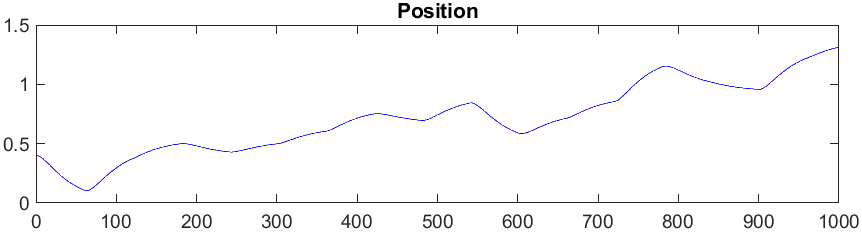
\includegraphics[width=130mm]{obr/position.png}
	\caption{Position of the pendulum $($LQR simulation$)$.}\label{lqrpos}
\end{figure}

\newpage
\subsection*{Simulation outputs}
Following the MATLAB simulation, the obtained results reveal distinctive patterns Fig. \ref{lqrpos}, \ref{lqrang}, \ref{lqrTorq}. Notably, each spike observed across all plots corresponds to the introduced disturbance. These disturbances were deliberately added to assess the robustness of the controller under varying conditions.

Figure \ref{lqrpos} shows the changing position of the pendulum carriage. Figure \ref{lqrang} shows the angle of the pendulum in radians and Fig. \ref{lqrTorq} shows the force i.e. torque applied, to move the pendulum. The full code can be found in appendix on the page \pageref{lqrSim.m}.



\begin{figure}[!tbh]
	\centering
	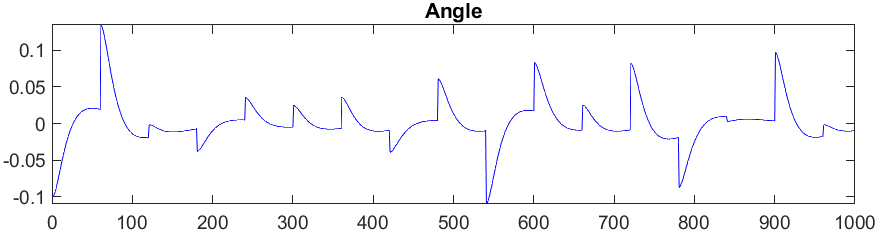
\includegraphics[width=130mm]{obr/lqrangle.png}
	\caption{Angle of the pendulum $($LQR simulation$)$.}\label{lqrang}
\end{figure}

\begin{figure}[!tbh]
	\centering
	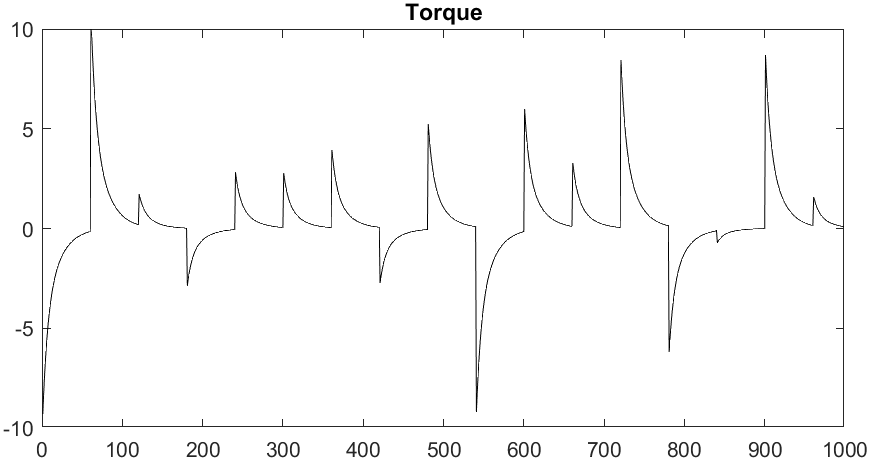
\includegraphics[width=130mm]{obr/torquelqr.png}
	\caption{Torque of the pendulum $($LQR simulation$)$.}\label{lqrTorq}
\end{figure}

Examining the plots, it becomes apparent that the angle of the pendulum Fig. \ref{lqrang} achieves stabilization in the unstable upright position within a maximum of 20 samples, depending on the level of disturbance introduced. However, it's important to note that the position of the pendulum Fig. \ref{lqrpos} does not attain stability; instead, it undergoes movement away from its initial 0 position $($when trying to control the pendulum angle$)$.

\subsection{Implementation}

\newpage
\section{Model predictive control (MPC)}
\subsection{Theory}
Model Predictive Control (MPC) represents an optimal control methodology where the computed control actions are designed to minimize a cost function for a constrained dynamical system over a finite, receding horizon. Its primary advantage over LQR control lies in its superior performance when the process encounters limitations \cite{zaklPredRiad}. However, it is acknowledged that MPC require a steeper learning curve and a more intricate implementation process. Often compared to playing chess, MPC depends on a deep understanding of the plant model and subsequent predictions of its behavior, recalculating the best possible output at each step \cite{zaklPredRiad}\cite{mpcLecture}.

In the MPC framework, the controller, at each time step, receives or estimates the current state of the plant. Based on this information, it computes a sequence of control actions that minimizes the cost over the specified horizon $($horizon can be sometimes infinite$)$ \cite{matlabMPC}\cite{zaklPredRiad}. This involves solving a constrained optimization problem, heavily relying on an internal plant model and dependent on the current system state. The controller then applies the first computed control action to the plant, disregarding the subsequent ones \cite{matlabMPC}. This iterative process repeats in each subsequent time step.

In practical applications, despite the finite horizon, MPC inherits several beneficial characteristics from traditional optimal control methodologies. It naturally accommodates multi-input multi-output (MIMO) plants, time delays, and possesses inherent robustness against model errors \cite{mpcLecture}. Furthermore, nominal stability can be assured by incorporating specific constraints. Overall, while MPC demands a more intricate knowledge of the system and involves a complex implementation, it gives big advantages in handling constraints and offering superior performance \cite{zaklPredRiad}.

In a mathematical way we can express MPC problem as: finding the best control sequence over a future horizon of N steps Eq. \ref{mpc1}
\begin{equation}\label{mpc1}
\underset{u_o,...,u_{N-1}}{min}\sum_{k=0}^{N-1}\left \| y_k-r(t) \right \|_{2}^{2}+\rho \left \| u_k-u_r(t) \right \|_{2}^{2}
\end{equation}
\begin{align}
s.t.	x_{k+1}&=f(x_k,u_k) \label{mpc2}\\ 
	y_k &=g(x_k) \nonumber
\end{align}
\begin{align}
	u_{min}\leq u_k\leq u_{max} \label{mpc3}\\
	y_{min}\leq y_k\leq y_{max} \nonumber
\end{align}
\begin{equation}\label{mpc4}
	x_o=x(t)
\end{equation}

Where Eq. \ref{mpc2} stands as the prediction model, Eq. \ref{mpc3} as constraints and Eq. \ref{mpc4} as state feedback \cite{mpcLecture}. 

\subsection{Simulation}

HOW WAS THE SIMULATION DONE\\

Following the MATLAB simulation, the obtained results reveal distinctive patterns Fig. \ref{mpcPos}, \ref{mpcAng}, \ref{mpcTor}. Notably, each spike observed across all plots corresponds to the introduced disturbance. These disturbances were deliberately added to assess the robustness of the controller under varying conditions.

Figure \ref{mpcPos} shows the changing position of the pendulum carriage. Figure \ref{mpcAng} shows the angle of the pendulum in radians and Fig. \ref{lqrTorq} shows the force i.e. torque applied, to move the pendulum. The full code can be found in appendix on the page \pageref{mpcSim.m}.

\begin{figure}[!tbh]
	\centering
	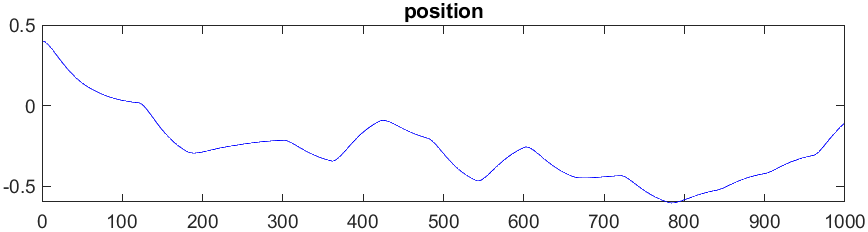
\includegraphics[width=150mm]{obr/mpcPos.png}
	\caption{Position of the pendulum $($MPC simulation$)$.}\label{mpcPos}
\end{figure}

\begin{figure}[!tbh]
	\centering
	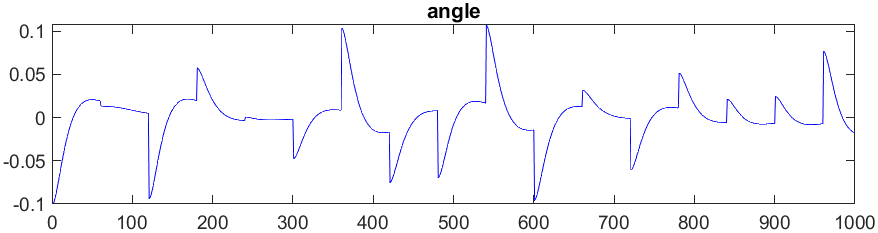
\includegraphics[width=150mm]{obr/mpcAng.png}
	\caption{Angle of the pendulum $($MPC simulation$)$.}\label{mpcAng}
\end{figure}

\begin{figure}[!tbh]
	\centering
	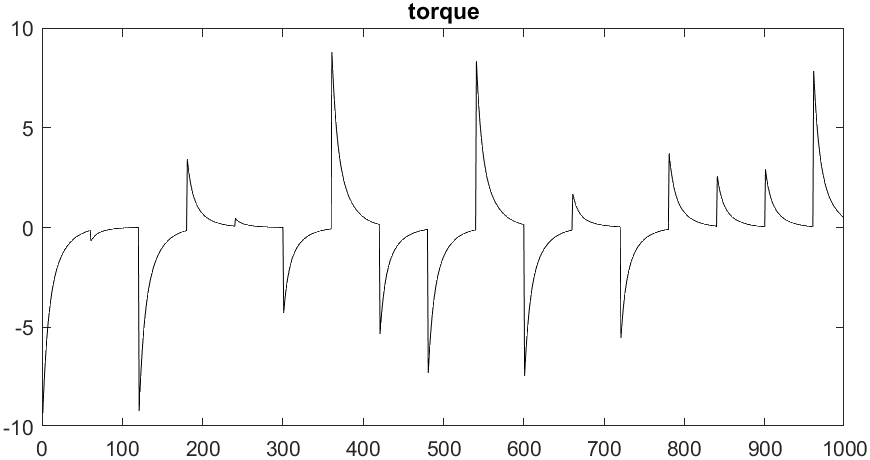
\includegraphics[width=150mm]{obr/mpcTor.png}
	\caption{Torque of the pendulum $($MPC simulation$)$.}\label{mpcTor}
\end{figure}

Examining the plots, it becomes apparent that the angle of the pendulum Fig. \ref{mpcAng} achieves stabilization in the unstable upright position within a maximum of 20 samples, depending on the level of disturbance introduced. However, it's important to note that the position of the pendulum Fig. \ref{mpcPos} does not attain stability; instead, it undergoes movement away from its initial 0 position $($when trying to control the pendulum angle$)$.

\subsection{Implementation}

\newpage
\section{Sliding mode control (SMC)}
\subsection{Theory}

Sliding mode control (SMC) is a nonlinear control methodology known for its impressive attributes such as precision, resilience, and straightforward tuning and application. It is applicable to both Single-Input Single-Output (SISO) and Multiple-Input Multiple-Output (MIMO) systems \cite{slidingLecture}\cite{Decarlo2008AQI}. The SMC consists of a two-part controller design. In the initial phase, an N-dimensional sliding surface must be designed where, by definition, the error asymptotically approaches zero. The subsequent phase is concerned with the selection of a control law, that will make the system states be attracted to the sliding surface.

The state-feedback control law is not a continuous function of time, rather, it can transition from one continuous structure to another based on the current position in the state space. The movement of the system as it glides along the boundaries of the control structures is referred to as a sliding mode, and the geometric locus comprising these boundaries is called the sliding surface \cite{wikiSMC}. SMC exhibits robustness against model uncertainties and disturbances. However, a significant drawback is the occurrence of chattering effects around the surface, which arises as a result of the switching of the control law. This is a common phenomenon in sliding mode control and is highly undesirable in practical applications due to increased control activity and the potential excitation of unmodeled high-frequency dynamics. Nevertheless, these issues can be mitigated or even avoided through the application of appropriate strategies \cite{slidingLecture}.

\subsection{Simulation}

The initial stage in simulating the sliding mode controller in MATLAB involved the creation of the sliding surface Eq. \ref{smcL1}. Afterwards, the calculation of the output estimate $\tau$ Eq. \ref{smcL5} needs to be done. 

\begin{align}
s &= (\frac{d}{dt}+e)\tilde{\alpha }+(\frac{d}{dt}+\beta )\tilde{\rho}=\dot{\tilde{\alpha }}+e\tilde{\alpha }+\dot{\tilde{\rho }}+\beta \tilde{\rho }=-\dot{\alpha }-e\alpha -\dot{\rho }-\beta \rho =0 \label{smcL1}\\
\dot{s} &=-\dot{\omega }-e\omega -\dot{v}-\beta v=0 \label{smcL2}\\
\dot{s} &=-\frac{}{}\varphi -\frac{}{}\alpha +\frac{}{}\tau +(\frac{}{}-e)\omega +\frac{}{}v-\frac{}{}\tau -\beta v \label{smcL3}\\
\dot{s} &= \label{smcL4}\\
\hat{\tau } &=\frac{j_a(m_\omega +m_e)}{m_el_{sp}-j_a}\left ( \frac{}{}+\frac{}{}-(\frac{}{}-e) -(\frac{}{}-\beta )v\right ) \label{smcL5}\\
\hat{\tau } &= \nonumber\\
\hat{\tau } &=12,335239v+68,877358\alpha -3,492138(0,125-e)\omega -3,492138(1,7568-\beta )v \nonumber
\end{align}

where $q_2$ stands for the pendulum angle, $\dot{q_2}$ is the angular velocity of the pendulum, $q_1$ is position of the base of the pendulum and $\dot{q_1}$ is the linear velocity of the base of the pendulum.

Following the MATLAB simulation, the obtained results reveal distinctive patterns Fig. \ref{posSmc}, \ref{angSmc}, \ref{torSmc}. Notably, each spike observed across all plots corresponds to the introduced disturbance. These disturbances were deliberately added to assess the robustness of the controller under varying conditions.

Figure \ref{posSmc} shows the changing position of the pendulum carriage. Figure \ref{angSmc} shows the angle of the pendulum in radians and Fig. \ref{torSmc} shows the force i.e. torque applied, to move the pendulum. The full code can be found in appendix on the page \pageref{smcSim}.

\begin{figure}[!tbh]
	\centering
	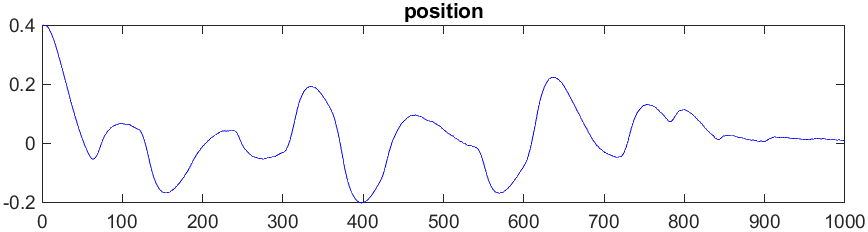
\includegraphics[width=150mm]{obr/posSmc.png}
	\caption{Position of the pendulum $($SMC simulation$)$.}\label{posSmc}
\end{figure}

\begin{figure}[!tbh]
	\centering
	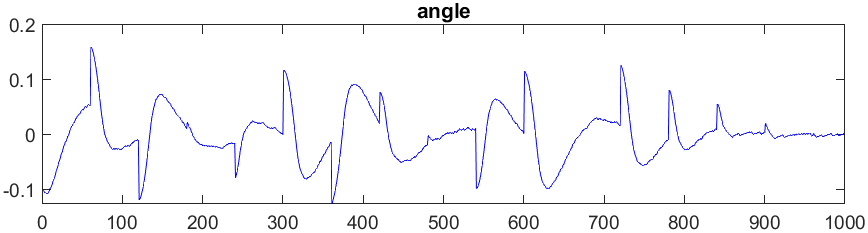
\includegraphics[width=150mm]{obr/angSmc.png}
	\caption{Angle of the pendulum $($SMC simulation$)$.}\label{angSmc}
\end{figure}

\begin{figure}[!tbh]
	\centering
	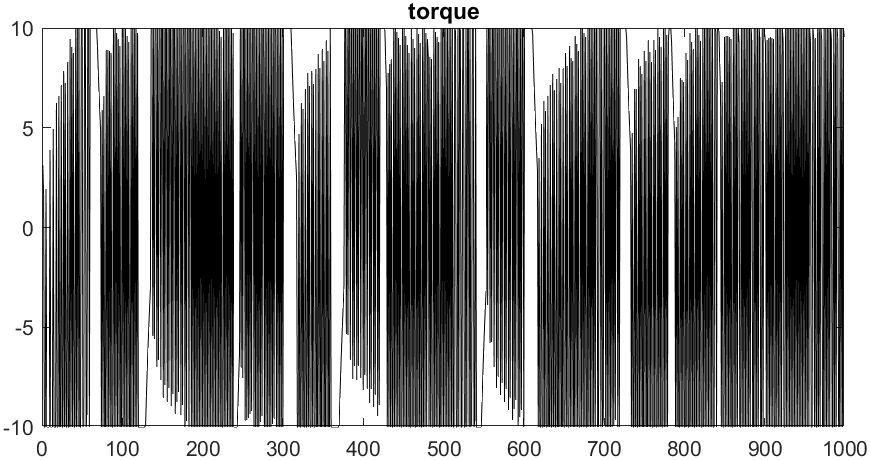
\includegraphics[width=150mm]{obr/torSmc.png}
	\caption{Torque of the pendulum $($SMC simulation$)$.}\label{torSmc}
\end{figure}

Examining the plots, it becomes apparent that the angle of the pendulum Fig. \ref{angSmc} achieves stabilization in the unstable upright position within a maximum of 40 samples, depending on the level of disturbance introduced. The position of the pendulum Fig. \ref{posSmc} attain stability within a maximum of 40 samples. We can clearly see the rapid switching of the control law on the Fig. \ref{torSmc}. 

\subsection{Implementation}

\newpage
\section{Fuzzy controller}
\subsection{Theory}
\subsection{Simulation}
\subsection{Implementation}

\newpage
\section{Impedance control}
\subsection{Theory}
\subsection{Simulation}
\subsection{Implementation}